\renewcommand{\theequation}{\theenumi}
\begin{enumerate}[label=\arabic*.,ref=\thesubsection.\theenumi]
\numberwithin{equation}{enumi}
%
%\item Draw the circumcircle of $\triangle ABC$, where 
%
\item $ABC$ is a triangle. Locate a point in the interior of $\triangle  ABC$ which is equidistant from all the vertices of $\triangle  ABC$.

\solution Let $\vec{O}$ be the desired point.  Then,
\begin{align}
\label{eq:circle_const_def}
\norm{\vec{A}-\vec{O}} = \norm{\vec{B}-\vec{O}} = 
\norm{\vec{C}-\vec{O}} = R
%\\
%\implies \norm{\vec{x}-\vec{O}}^2 &=\brak{\vec{x}-\vec{O}}^T\brak{\vec{x}-\vec{O}} = R^2
\end{align}
From \eqref{eq:circle_const_def},
\begin{align}
\label{eq:circle_const_AB}
\norm{\vec{A}-\vec{O}}^2 - \norm{\vec{B}-\vec{O}}^2  = 0
\end{align}
\begin{multline}
\implies \brak{\vec{A}-\vec{O}}^T\brak{\vec{A}-\vec{O}} 
\\
- \brak{\vec{B}-\vec{O}}^T\brak{\vec{B}-\vec{O}} = 0
\end{multline}
%
which can be simplified as
\begin{align}
\label{eq:circle_const_chord_ab}
\brak{\vec{A}-\vec{B}}^T\vec{O} =   \frac{\norm{\vec{A}}^2- \norm{\vec{B}}^2}{2}
\end{align}
Similarly,
\begin{align}
\label{eq:circle_const_chord_bc}
\brak{\vec{B}-\vec{C}}^T\vec{O} =   \frac{\norm{\vec{B}}^2- \norm{\vec{C}}^2}{2}
\end{align}
%
From \label{eq:circle_const_chord_ab} and \label{eq:circle_const_chord_ab}, $\vec{O}$ can be computed.
%
A circle with centre $\vec{O}$ can be drawn through $\vec{A}, \vec{B}, \vec{C}$.  This circle is known as the {\em circumcircle}.  
The following code plots Fig. \ref{fig:circle_const_ccircle}
\begin{lstlisting}
codes/circle/circle_const_ccircle.py
\end{lstlisting}
\begin{figure}[!ht]
\includegraphics[width=\columnwidth]{./circle/figs/circle_const_ccircle.eps}
\caption{}
\label{fig:circle_const_ccircle}
\end{figure}

\item  In a triangle locate a point in its interior which is equidistant from all the sides of the triangle.
%
\item Draw a circle with centre $\vec{B}$ and radius 6.  If $\vec{C}$ be  a point 10 units  away from its 
centre, construct the pair of tangents $AC$ and $CD$ to the 
circle.
\\
\solution The tangent is perpendicular to the radius.
%
From the given information, in $\triangle ABC, AC \perp AB, a = 
10$ and $c = 6$.
\begin{align}
b =  \sqrt{a^2-c^2}
\end{align}
The following code plots Fig. \ref{fig:circle}
\begin{lstlisting}
codes/circle/draw_circle_eg.py
\end{lstlisting}
\begin{figure}[!ht]
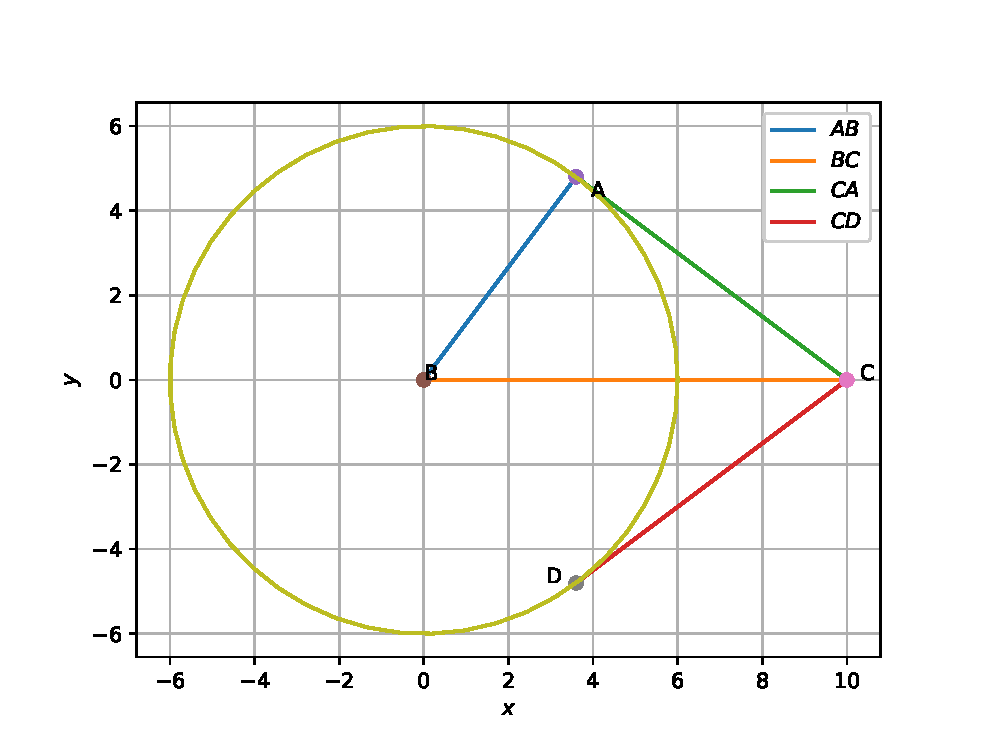
\includegraphics[width=\columnwidth]{./circle/figs/circle.eps}
\caption{}
\label{fig:circle}
\end{figure}
\item Draw a circle of radius 3.  Mark any point $\vec{A}$ on the circle, point  $\vec{B}$ inside the circle  and point  $\vec{C}$ outside the circle.
\\
\solution 
For any angle $\theta$, a point on the circle with radius 3 has coordinates
\begin{align}
3\myvec{\cos \theta\\ \sin\theta}
\end{align}
